\documentclass[10pt,a4paper]{article}

\usepackage{enumerate}
\usepackage{indentfirst}
%\usepackage{arev}
\usepackage{amsthm,amsfonts,amsmath,amssymb}
\usepackage[brazilian]{babel}
\usepackage[T1]{fontenc}
\usepackage{txfonts}
%\usepackage{ulem}
%\usepackage[latin1]{inputenc}
\usepackage[utf8]{inputenc}
%\usepackage{multicol}
\usepackage{setspace}
%\usepackage{natbib}
\usepackage[usenames,dvipsnames]{xcolor} 
\usepackage{pgf,tikz}
%\usepackage{algpseudocode}
\usepackage{float}
\usepackage{graphicx}
\usepackage{subfigure}
\usepackage{wrapfig}
%\usepackage{listings}
%\usepackage[linesnumbered, ruled, portuguese]{algorithm2e}
\usepackage{multirow}
%\usepackage{verbatim}
%\usepackage[active,tightpage]{preview}
%\PreviewEnvironment{tikzpicture}
%\setlength\PreviewBorder{5pt}
\usepackage{geometry}
\usepackage[pdftex]{hyperref}
\usepackage{listings}
\usepackage[normalem]{ulem}
\usepackage{enumitem}
\lstdefinelanguage{VHDL}{
  morekeywords=[1]{
abs,access,after,alias,all,and,architecture,array,assert,attribute,begin,block,body,buffer,bus,case
component,configuration,constant,disconnect,downto,else,elsif,end,entity,exit,file,for,function,generate,
generic,group,guarded,if,impure,in,inertial,inout,is,label,library,linkage,literal,loop,map,mod,
nand,new,next,nor,not,null,of,on,open,or,others,out,package,port,postponed,procedure,process,pure,
range,record,register,reject,return,rol,ror,select,severity,signal,shared,sla,sli,sra,srl,subtype,then,
to,transport,type,unaffected,units,until,use,variable,wait,when,while,with,xnor,xor,
ABS,ACCESS,AFTER,ALIAS,ALL,AND,ARCHITECTURE,ARRAY,ASSERT,ATTRIBUTE,BEGIN,BLOCK,BODY,BUFFER,BUS,CASE
COMPONENT,CONFIGURATION,CONSTANT,DISCONNECT,DOWNTO,ELSE,ELSIF,END,ENTITY,EXIT,FILE,FOR,FUNCTION,GENERATE,
GENERIC,GROUP,GUARDED,IF,IMPURE,IN,INERTIAL,INOUT,IS,LABEL,LIBRARY,LINKAGE,LITERAL,LOOP,MAP,MOD,
NAND,NEW,NEXT,NOR,NOT,NULL,OF,ON,OPEN,OR,OTHERS,OUT,PACKAGE,PORT,POSTPONED,PROCEDURE,PROCESS,PURE,
RANGE,RECORD,REGISTER,REJECT,RETURN,ROL,ROR,SELECT,SEVERITY,SIGNAL,SHARED,SLA,SLI,SRA,SRL,SUBTYPE,THEN,
TO,TRANSPORT,TYPE,UNAFFECTED,UNITS,UNTIL,USE,VARIABLE,WAIT,WHEN,WHILE,WITH,XNOR,XOR
  },
  morekeywords=[2]{
    STD_LOGIC_VECTOR,STD_LOGIC,IEEE,STD_LOGIC_1164,
    NUMERIC_STD,STD_LOGIC_ARITH,STD_LOGIC_UNSIGNED,std_logic_vector,
    std_logic
  },
  morecomment=[l]{--}
}

\colorlet{keyword}{blue!100!black!80}
\colorlet{STD}{Lavender}
\colorlet{comment}{green!80!black!90}
\lstdefinestyle{vhdl}{
  language     = VHDL,
  basicstyle   = \footnotesize \ttfamily,
  keywordstyle = [1]\color{keyword}\bfseries,
  keywordstyle = [2]\color{STD}\bfseries,
  commentstyle = \color{comment},
  breaklines=true,                % sets automatic line breaking
  tabsize=3                                % sets default tabsize to 2 spaces
}

\geometry{a4paper,inner=2.0cm,outer=2.0cm,top=2.0cm,bottom=2.0cm}


\newcommand{\pr}{\hspace*{0.6cm}}
\newcommand{\vesp}{\vspace*{.3cm}}

\newcommand{\sen}{\mbox{\,sen}}
\newcommand{\cotg}{\mbox{\,cotg\,}}
\newcommand{\tg}{\mbox{\,tg\,}}
\newcommand{\cose}{\mbox{\,cos\,}}
\newcommand{\expo}{\mbox{\,e\,}}
\newcommand{\logg}{\mbox{\,log}}
\newcommand{\Sum}{\displaystyle\sum}
\newcommand{\Prod}{\displaystyle\prod}
\newcommand{\Int}{\displaystyle\int}
\newcommand{\dint}{\, \mathrm{d}}
\newcommand{\Lim}{\displaystyle \lim}
\newcommand{\Frac}{\displaystyle\frac}

\newcommand{\Nc}{N_{cont}}
\newcommand{\Ni}{N_{int}}
\newcommand{\Ne}{N_{estrela}}

\newcommand{\Dparc}[2]{\frac{\partial #1}{\partial #2}}
\newcommand{\Dparcn}[3]{\frac{\partial^#3 #1}{\partial^#3 #2}}

\newcommand{\R}{\mathbb{R}}
\newcommand{\V}{\mathcal{V}}
\newcommand{\I}{I_u}
\newcommand{\Fi}{\varphi}
\newcommand{\se}{\mbox{ se }}
\newcommand{\norma}[1]{\left|\left| #1 \right|\right|}
\newcommand{\sistema}[1]{ \left\{ #1 \right. }

\newtheorem{exemplo}{\pr \sc Exemplo}[section]%[chapter]
\newtheorem{defi}{\pr \sc Defini\c{c}\~ao}[section]%[chapter]
\newtheorem{obs}{\pr \sc Observa\cao}[section]%[chapter]
\newtheorem{teor}{\pr \sc Teorema}[section]%[chapter]
\newtheorem{lema}{\pr \sc Lema}[section]%[chapter]
\newtheorem{prop}{\pr \sc Proposi\cao}[section]%[chapter]
\newtheorem{exercise}{\pr \sc Exerc\'\i cios}[section]%[chapter]
\newtheorem{alg}{\pr Algoritmo}[section]%[chapter]

\setlength{\columnsep}{1cm}

\setlength{\columnsep}{1cm}

\lstset{language=VHDL}

\lstdefinestyle{customc}{
  belowcaptionskip=1\baselineskip,
  breaklines=true,
  xleftmargin=\parindent,
  language=C,
  showstringspaces=false,
    keywordstyle=\bfseries\color{green!40!black},
  commentstyle=\itshape\color{purple!40!black},
  identifierstyle=\color{blue},
  stringstyle=\color{orange},
} 
\allowdisplaybreaks
%basicstyle=\footnotesize\ttfamily,

\lstset{escapechar=@,style=vhdl}
\addto\captionsbrazilian{% Replace "english" with the language you use
  \renewcommand{\contentsname}%
    {Tabela de Conteúdo}%
}
\newcommand*\NewPage{\newpage\null\thispagestyle{empty}\newpage}
\begin{document}
\thispagestyle{empty}
\begin{center}
	UNIVERSIDADE DE SÃO PAULO – USP
	
	INSTITUTO DE CIÊNCIAS MATEMÁTICAS E DE COMPUTAÇÃO
	
	DEPARTAMENTO DE SISTEMAS DE COMPUTAÇÃO
	
	\vspace{7cm}
	
	\Large{\textbf{RELATÓRIO}}
	 
	\Large{\textbf{Trabalho Prático 1}}\\
	
	\vspace{6cm}
	
	Adams Vietro Codignotto da Silva - $6791943$ \\ 
	Gabriel Estrela - $8124138$\\
	Luiz Dorici - $4165850$ \\
	Maiser J. Alves	- $6309717$\\
	
	
	\vspace{6cm}
	
	São Carlos
	
	2015
\end{center}

\NewPage
\pagenumbering{arabic}

\tableofcontents

\newpage
\section{Resultados}
\begin{figure}[H]
\subsection{Base Binária}
\begin{minipage}[t]{.5\textwidth}
\subsubsection{para Octal}
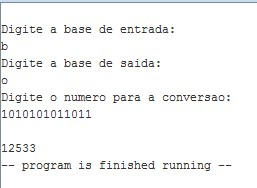
\includegraphics[width=\textwidth]{BO.jpg}
\end{minipage}
\begin{minipage}[t]{.5\textwidth}
\subsubsection{para Decimal}
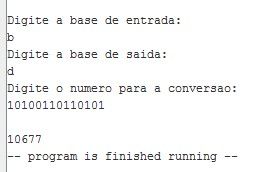
\includegraphics[width=\textwidth]{BD.jpg}
\end{minipage}
\begin{minipage}[t]{.5\textwidth}
\subsubsection{para Hexadecimal}
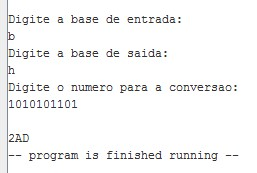
\includegraphics[width=\textwidth]{BH.jpg}
\end{minipage}
\begin{minipage}[t]{.5\textwidth}
\subsubsection{Verificação de Binário}
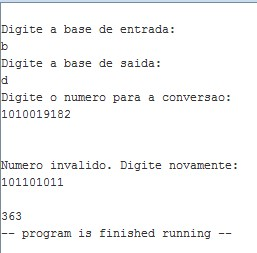
\includegraphics[width=\textwidth]{BinFail.jpg}
\end{minipage}
\end{figure}
\newpage
\subsection{Base Octal}
\begin{figure}[H]
\begin{minipage}[t]{.5\textwidth}
\subsubsection{para Binaria}
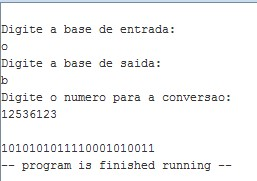
\includegraphics[width=\textwidth]{OB.jpg}
\end{minipage}
\begin{minipage}[t]{.5\textwidth}
\subsubsection{para Decimal}
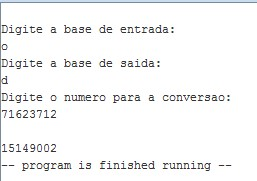
\includegraphics[width=\textwidth]{OD.jpg}
\end{minipage}
\begin{minipage}[t]{.5\textwidth}
\subsubsection{para Hexadecimal}
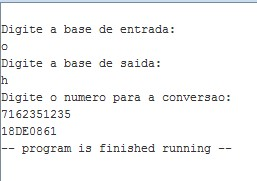
\includegraphics[width=\textwidth]{OH.jpg}
\end{minipage}
\begin{minipage}[t]{.5\textwidth}
\subsubsection{Verificação de Octal}
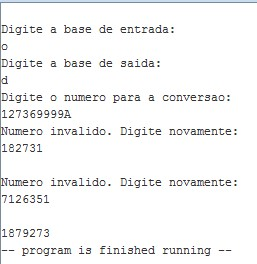
\includegraphics[width=\textwidth]{OctalFail.jpg}
\end{minipage}
\end{figure}
\newpage
\subsection{Base Decimal}
\begin{figure}[H]
\begin{minipage}[t]{.5\textwidth}
\subsubsection{para Binaria}
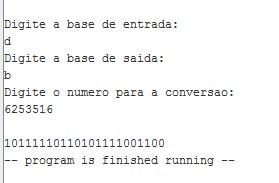
\includegraphics[width=\textwidth]{DB.jpg}
\end{minipage}
\begin{minipage}[t]{.5\textwidth}
\subsubsection{para Octal}
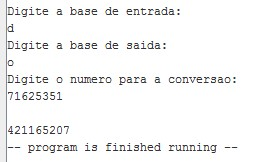
\includegraphics[width=\textwidth]{DO.jpg}
\end{minipage}
\begin{minipage}[t]{.5\textwidth}
\subsubsection{para Hexadecimal}
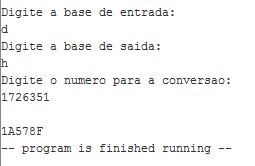
\includegraphics[width=\textwidth]{DH.jpg}
\end{minipage}
\begin{minipage}[t]{.5\textwidth}
\subsubsection{Verificação de Decimal}
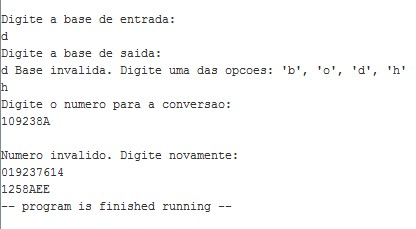
\includegraphics[width=\textwidth]{DecFail.jpg}
\end{minipage}
\end{figure}
\newpage
\subsection{Base Hexadecimal}
\begin{figure}[H]
\begin{minipage}[t]{.5\textwidth}
\subsubsection{para Binaria}
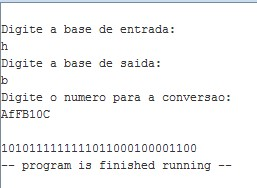
\includegraphics[width=\textwidth]{HB.jpg}
\end{minipage}
\begin{minipage}[t]{.5\textwidth}
\subsubsection{para Octal}
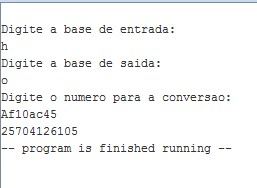
\includegraphics[width=\textwidth]{HO.jpg}
\end{minipage}
\begin{minipage}[t]{.5\textwidth}
\subsubsection{para Decimal}
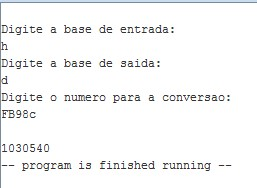
\includegraphics[width=\textwidth]{HD.jpg}
\end{minipage}
\begin{minipage}[t]{.5\textwidth}
\subsubsection{Verificação de Hexadecimal}
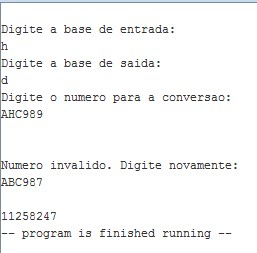
\includegraphics[width=\textwidth]{HexFail.jpg}
\end{minipage}
\end{figure}
\newpage
\section{Observações}
\begin{enumerate}
\item É tratado a possibilidade de digitar, em hexa, tanto letras maiúsculas quanto minúsculas.
\item Quando é oferecida a escolha de base, apenas letras minúsculas são verifiadas.
\end{enumerate}
\end{document}